\documentclass[12pt]{article}
\usepackage[a4paper, total={7.5in, 11in}]{geometry}
%\usepackage{array}
\usepackage{graphicx, subfig, wrapfig, fancyhdr, lastpage, multicol ,color}
\newcommand\headerMe[2]{\noindent{}#1\hfill#2}
\usepackage[mathscr]{euscript}
\usepackage{tabularray}

\setlength{\columnseprule}{1pt}
\def\columnseprulecolor{\color{blue}}


\pagestyle{fancy}
\fancyhf{}

\cfoot{ \vspace{-0.8cm}\em{Page \thepage \hspace{1pt} / \pageref{LastPage}}}
\begin{document}

\headerMe{Royaume du Maroc}{année scolaire \emph{2024-2025}}\\
\headerMe{Ministère de l'Éducation nationale, }{  Professeur :\emph{Zakaria Haouzan}}\\
\headerMe{du Préscolaire et des Sports}{Établissement : \emph{Lycée SKHOR qualifiant}}\\

\begin{center}
Devoir Surveillé  N°3 - semestre 02 \\
    2ème année baccalauréat Sciences Mathématiques\\
Durée 2h00
\\
    \vspace{.2cm}
\hrulefill
\Large{Chimie 7pts/42min}
\hrulefill\\

	\emph{Toutes les solutions sont prises à 25°c, et $K_e=10^{-14}$. }
\end{center}
%end Headerss------------------------
%__________________Chimie ______________________-
%%%%%%%+_+_+_+_+_+_+_+_+_Partie1

 \section*{Partie 1 :Amines et composés apparentés \dotfill(7pts) }

 \emph{Les amines sont des composés organiques qui se caractérisent par des solutions
aqueuses basique. On s’intéresse à l’étude d’une solution aqueuse d’une amine A de
formule $C_2H_5NH_2.$ }

On prépare une solution S0 de cette amine de concentration $C_0=2.10^{-2} mol/L$ et de $pH_0=11,55$ à 25°c.

\begin{tblr}{c|[dashed]l}
	1  & {\textbf{1.1. }Ecrire l’équation de réaction de l’amine A avec l’eau, et dresser le tableau
	d’avancement\\pour un volume V.} \\
	0.5  & \textbf{1.2. }Calculer le taux d’avancement final de la réaction. Conclure.\\
	1  & \textbf{1.3. }Calculer la valeur de $pK_A$ du couple acide/base de l’amine A. \\
	1.5  & {\textbf{1.4. }On dilue la solution $S_0$, pour obtenir une solution $S_1$ de concentration
	$C_1=10^{-2} mol/L$ . \\En négligeant la dissolution de la base avec l’eau, montrer que le
	pH de la solution $S_1$ peut\\ s’écrire sous la forme : $pH = 7 + \frac{1}{2}.(pK_A + log(C_1)$.
Calculer $pH_1$. } \\
\end{tblr}

\textbf{2.} On prend $V_1=10mL$ de la solution $S_1$, et on procède au dosage avec une solution
aqueuse d’acide chlorhydrique $(H_3O^+_{(eq)} + Cl^-)$ de concentration $C_2=10^{-2} mol/L$.
L’évolution de la valeur de pH du mélange au cours du dosage, est représentée par la
courbe de la figure .

\begin{center}
  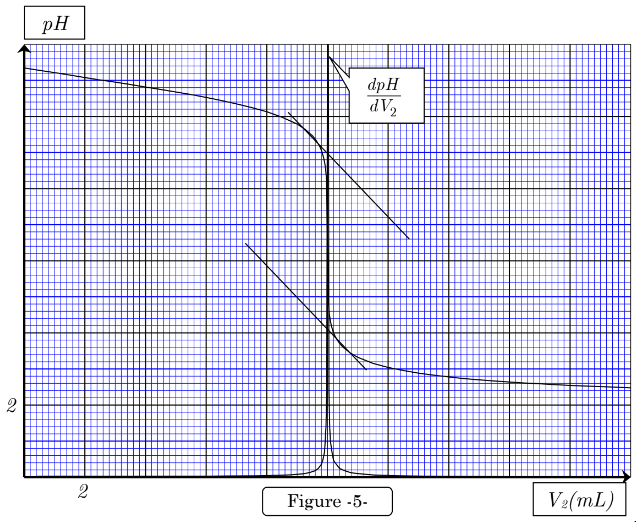
\includegraphics[width=0.6\textwidth]{./img/chimie00.png}
\end{center}


\begin{tblr}{c|[dashed]l}
	0.75  & {\textbf{2.1. }Ecrire l’équation de réaction du dosage, et calculer sa constante d’équilibre.
\\Que peut-on dire de la nature de cette réaction ? } \\
	0.75  & {\textbf{2.2. }Déterminer les coordonnées du point d’équivalence, puis vérifier la valeur de la
$C_1$. }\\
	1.5  & {\textbf{2.3. }Calculer les concentrations de l’amine A et de son acide conjugué lorsqu’on a
versé \\un volume $V_2=16ml$ de la solution titrante. En déduire le pourcentage de
chacun. } \\
\end{tblr}
%\hrulefill
%\Large{Physique 13pts/78min}
%\hrulefill\\
\begin{center}
    %\vspace{.60cm}
\hrulefill
\Large{Physique 13pts}
\hrulefill\\
    \emph{Les deux parties sont indépendantes}
\end{center}


\section*{Partie 1:Electricité (1) \dotfill(7pts) }

\begin{wrapfigure}[3]{r}{0.25\textwidth}
	\vspace{-1cm}
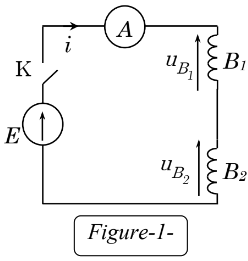
\includegraphics[width=0.9\linewidth]{./img/phys00.png} 
\end{wrapfigure}

On réalise le circuit électrique représenté dans
la figure-1- comportant :
\begin{itemize}
	\item Un générateur de force électromotrice E.
	\item Une bobine d’inductance $L_1$ et de résistance
interne $r_1$.
\item Une bobine d’inductance $L_2$ et de résistance
interne $r_2$.
\item Un ampèremètre et un interrupteur K.
On ferme K à t=0.
\end{itemize}

\begin{tblr}{c|[dashed]l}
	0.5  & {\textbf{1. }Montrer que l’équation différentielle vérifié par l’intensité du courant i(t)
	s’écrit \\sous la forme : $i + \tau.\frac{di}{dt} = \alpha$ \\
	Avec $\tau$ et $\alpha$ , des constantes dont on déterminera les expressions.
	}\\
	
	1 & {\textbf{2. }La solution de cette équation s’écrit sous la forme : $i(t) =A.e^{-\lambda.t} + B$. En
utilisant les \\conditions initiales et les caractéristiques du régime permanant,
trouver les expressions des \\constantes A et B.  } \\
	\end{tblr}

\textbf{II. }La courbe de la figure -2 montre les variations de l’intensité du courant
i(t), et la figure -3-, celles des tensions ${u_B}_1(t)$ et ${u_B}_2(t)$ aux bornes des bobines.

\begin{center}
  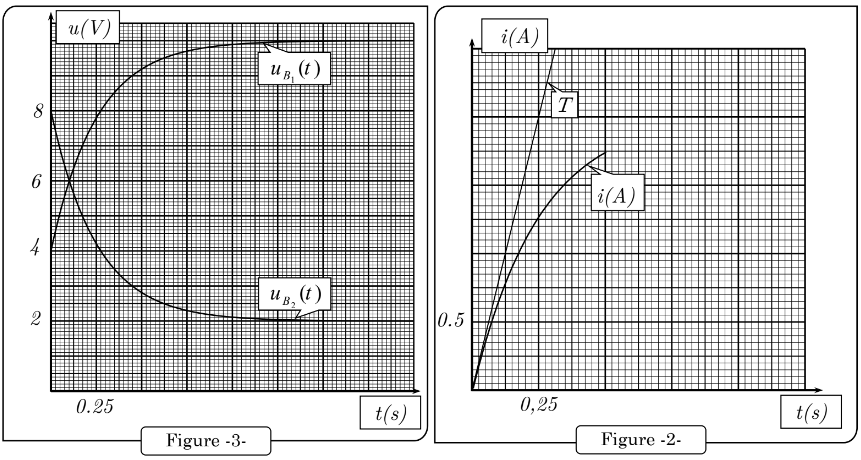
\includegraphics[width=0.7\textwidth]{./img/phys01.png}
\end{center}
\begin{tblr}{c|[dashed]l}
	0.5  & {\textbf{3. }Montrer que E=12V. }\\

	0.5 & {\textbf{4. }Trouver l’expression de $\frac{di}{dt}(t = 0)$, à $t=0$ en fonction de E, $L_1$, et $L_2$}.\\
	
	1 & {\textbf{5. }La droite T dans la figure-2, représente la tangente à la courbe i(t) à t=0.
	Trouver graphiquement \\la valeur $\frac{di}{dt}(t=0)$, et en déduire la valeur de $L_1+L_2$. }.\\

	0.75 & {\textbf{6. }Montrer que $u_{B1}(t = 0) = \frac{L_1}{L_1 + L_2}.E $ et $u_{B2}(t = 0) = \frac{L_2}{L_1 + L_2}.E $\\
	En utilisant les courbes de la figures -3, trouver les valeurs de $L_1$ et $L_2$.
	}.\\

	0.75 & {\textbf{7. }Montrer qu’en régime permanant, les tensions  $u_{B1}(\infty) = \frac{r_1}{r_1 + r_2}.E $ et $u_{B2}(\infty) = \frac{r_2}{r_1 + r_2}.E $  }.\\
	
	0.5 & {\textbf{8. }En régime permanant, l’ampèremètre affiche la valeur $2A$. Calculer les valeurs de $r_1$ et $r_2$. }.\\
	
	1.5 & {\textbf{9. }L’expression de la tensions $u{B_1}(t)$ s’écrit sous la forme : $u_{B_1} = C + D.e^{\frac{-t}{\tau}}$ \\Trouver les expressions des deux constante C et D. }.\\

\end{tblr}


\section*{Partie 2 : Electricité(2)De l’énergie solaire à l’énergie électrique  \dotfill(6pts) }

\begin{wrapfigure}[18]{r}{0.4\textwidth}
  \begin{center}
    
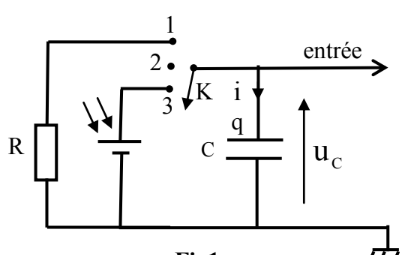
\includegraphics[width=0.3\textwidth]{./img/circuit00.png} 
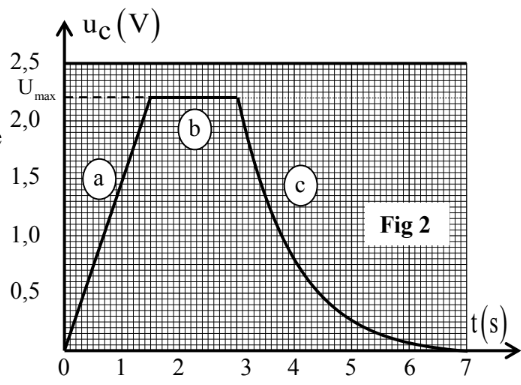
\includegraphics[width=0.4\textwidth]{./img/courbe00.png} 

  \end{center}
\end{wrapfigure}


\emph{On peut transformer l’énergie solaire en ’énergie électrique et la stocker dans des batteries
d’accumulateurs ou dans des condensateurs et l’utiliser au besoin.
L’objectif de cet exercice est l’étude de la charge d’un condensateur au moyen d’un panneau
solaire, puis au moyen d’un échelon de tension ascendant.}

Pour comparer l’évolution de la tension aux bornes du condensateur au cours de sa charge à l’aide d’un
panneau solaire et à l’aide d’un échelon de tension ascendant , Ahmed et Myriam ont réalisé les deux
expériences suivantes :



\textbf{I- Charge d’un condensateur au moyen d’un panneau solaire}

Le panneau solaire se comporte, lorsqu’il est exposé au soleil,
comme un générateur donnant un courant d’intensité
constante $i = I_0$ tant que la tension entre ses bornes est inferieure 
à une tension maximale $u_{max} $=$2,25V$

Myriam a réalisé le montage représenté dans la figure 1,
comportant un panneau solaire et un condensateur de capacité $C=0,10F$
et un conducteur ohmique de résistance $R=10\Omega$
et un interrupteur K.

A l’aide d’un dispositif d’acquisition, Myriam a
visualisé la tension $u_C$ aux bornes du condensateur
en basculant l’interrupteur trois fois successives ;

Elle obtient le graphe représentée dans la figure 2 qui
comprend trois parties (a),(b) et (c) selon la position de
l’interrupteur .

\begin{tblr}{c|[dashed]l}
1  & {\textbf{1.1. } Associer chacune des parties du graphe à
la position correspondant de L’interrupteur K.\\
Déduire, en exploitant le graphe, la valeur de
l’intensité $I_0$
au cours de la charge.}\\

  1  & {\textbf{1.2. } Trouver l’expression de l’équation différentielle
  vérifiée par la charge q(t) du condensateur:\\ (au cours de la charge) et (au cours de la decharge)}\\

  1  & {\textbf{1.3. } L’expression de la tension $u_C$ au cours de la décharge s’exprime par la fonction \\$u_C(t) = U_{max}.e^{-(\frac{t-3}{\tau})}$ avec $\tau$ la constante du temps du circuit utilisé.\\ En déduire l’expression de l’intensité  i(t) et dessiner, sans échelle, l’allure de la courbe représentant \\i(t) en respectant les conventions et l’origine du temps ( figures 1 et 2)}\\
\end{tblr}



\textbf{II- Charge d’un condensateur au moyen d’un échelon de tension ascendant}

\begin{wrapfigure}[15]{r}{0.36\textwidth}
  \begin{center}
    \vspace{-1cm}
    
  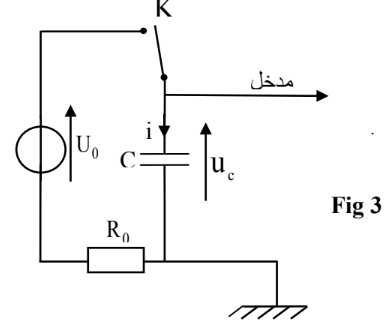
\includegraphics[width=0.3\textwidth]{./img/circuit01.png} 
    \vspace{-0.6cm}
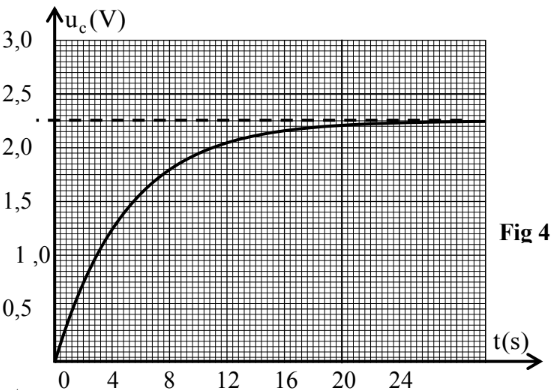
\includegraphics[width=0.4\textwidth]{./img/courbe01.png} 

  \end{center}
\end{wrapfigure}


Ahmed a réalisé le montage représenté dans la figure 3. Pour charger le condensateur précédent de capacité
C il a utilisé un générateur donnant une tension constante $U_0 = 2,25V$
A l’instant $t=0$,
il ferme le circuit ; alors le condensateur se charge à travers la résistance
$R_0=50\Omega$

A l’aide d’un dispositif d’acquisition, il visualise l’évolution de la tension
$u_C$ aux bornes du condensateur.

Il obtient la courbe représentée dans la figure 4.


\begin{tblr}{c|[dashed]l}
0,5  & {\textbf{2.1. } Établir l’équation différentielle que vérifie
la tension $u_C$ au cours de la charge} \\
0,5  & {\textbf{2.2. } La solution de l’équation différentielle s’écrit sous \\la forme $u_C(t) = A.e^{\frac{-t}{\tau}} + B$ avec $\tau$
\\la constante de
temps du circuit utilisé.

A l’aide de la courbe (fig4 ), \\calculer la valeur des deux constantes A et B .
} \\
  1  & {\textbf{2.3. } Trouver l’expression de l’intensité du courant

  $i(t)$ en fonction du temps au cours de la charge ,

  Et dessiner, sans échelle, l’allure de la courbe représentant
  \\$i(t)$
en respectant les conventions et
l’origine du temps t.} \\
1  & {\textbf{2.4 } Calculer la valeur de la résistance $R_0$ que doit utiliser \\Ahmed pour que son condensateur se
charge totalement pendant la même durée de la charge \\totale du condensateur de Myriam, sachant
que la durée de la charge totale est de l’ordre de $5.\tau$.} \\

\end{tblr}
\end{document}
